%%
%% This is file `sample-lualatex.tex',
%% generated with the docstrip utility.
%%
%% The original source files were:
%%
%% samples.dtx  (with options: `sigconf')
%% 
%% IMPORTANT NOTICE:
%% 
%% For the copyright see the source file.
%% 
%% Any modified versions of this file must be renamed
%% with new filenames distinct from sample-lualatex.tex.
%% 
%% For distribution of the original source see the terms
%% for copying and modification in the file samples.dtx.
%% 
%% This generated file may be distributed as long as the
%% original source files, as listed above, are part of the
%% same distribution. (The sources need not necessarily be
%% in the same archive or directory.)
%%
%% The first command in your LaTeX source must be the \documentclass command.
\documentclass[sigconf]{acmart}
\settopmatter{printacmref=false}  % Removes citation information below abstract
\renewcommand\footnotetextcopyrightpermission[1]{} % removes footnote with conference information in first column
%\pagestyle{plain} % removes running headers
%\documentclass[]{paper}

%%%% As of March 2017, [siggraph] is no longer used. Please use sigconf (above) for SIGGRAPH conferences.

%%%% As of May 2020, [sigchi] and [sigchi-a] are no longer used. Please use sigconf (above) for SIGCHI conferences.

%%%% Proceedings format for SIGPLAN conferences 
% \documentclass[sigplan, anonymous, review]{acmart}

%%%% Proceedings format for conferences using one-column small layout
% \documentclass[acmsmall,review]{acmart}

%%
%% \BibTeX command to typeset BibTeX logo in the docs
\AtBeginDocument{%
  \providecommand\BibTeX{{%
    \normalfont B\kern-0.5em{\scshape i\kern-0.25em b}\kern-0.8em\TeX}}}



%%
%% Submission ID.
%% Use this when submitting an article to a sponsored event. You'll
%% receive a unique submission ID from the organizers
%% of the event, and this ID should be used as the parameter to this command.
%%\acmSubmissionID{123-A56-BU3}

%%
%% The majority of ACM publications use numbered citations and
%% references.  The command \citestyle{authoryear} switches to the
%% "author year" style.
%%
%% If you are preparing content for an event
%% sponsored by ACM SIGGRAPH, you must use the "author year" style of
%% citations and references.
%% Uncommenting
%% the next command will enable that style.
%%\citestyle{acmauthoryear}

%%
%% end of the preamble, start of the body of the document source.
\setcopyright{none}
\begin{document}

%%
%% The "title" command has an optional parameter,
%% allowing the author to define a "short title" to be used in page headers.
\title{Least Privilege CTF}

%%
%% The "author" command and its associated commands are used to define
%% the authors and their affiliations.
%% Of note is the shared affiliation of the first two authors, and the
%% "authornote" and "authornotemark" commands
%% used to denote shared contribution to the research.
\author{Wenjing Wu}
\email{wwu@pdx.edu}
\affiliation{%
  \institution{Portland State University}
  \streetaddress{1900 SW 4th Ave}
  \city{Portland}
  \state{Oregon}
  \postcode{97201}
}



%%
%% By default, the full list of authors will be used in the page
%% headers. Often, this list is too long, and will overlap
%% other information printed in the page headers. This command allows
%% the author to define a more concise listfocus
%% of authors' names for this purpose.
%% \renewcommand{\shortauthors}{Trovato and Tobin, et al.}

%%
%% The abstract is a short summary of the work to be presented in the
%% article.
\begin{abstract}
 As more businesses integrating into the cloud environment, the importance of following the principle of least privilege (PoLP) to mitigate security risks significantly increases. The fact that both identity and access management (IAM) and infrastructure itself in cloud environments are sophisticated, and the lack of CTF (Capture-the-Flag) exercises pivot around IAM best practices make the task of understanding the concepts and following PoLP onerous. This paper describes Least Privilege CTF, a series of Google Cloud based labs that can be quickly deployed at minimal cost, to assist comprehension and illustrate the process of implementing PoLP.
\end{abstract}



%%
%% Keywords. The author(s) should pick words that accurately describe
%% the work being presented. Separate the keywords with commas.
\keywords{cloud security, CTF, least privilege, IAM}


%%
%% This command processes the author and affiliation and title
%% information and builds the first part of the formatted document.
\maketitle
\pagestyle{plain}
%\fancyfoot{}
%\thispagestyle{empty}

\section{Introduction}
%% subsections are used to keep track of outlines and will be removed after..

Advantages bestowed by cloud technologies, such as efficiency, agility, scalability and cost savings, are crucial for business success in today’s market. According to the 2020 Flexera State of the Cloud Report \cite{Flexera2020}, enterprises are running 48\% of their workloads and storing 45\% of their data in public clouds and planning to increase workload and data-related cloud utilization by 9\% and 8\% respectively over the next 12 months. 

Clouds allow organizations to reduce startup costs and maintenance tasks in infrastructure (hardware and network) layers through virtualization. However, integration, both between cloud services and legacy systems and between various services from different cloud resources and platforms, is quite complex \cite{Baron2019}. 
The findings in the same Flexera report \cite{Flexera2020} indicate that 93\% of enterprises are embracing multi-cloud solutions (involving multiple public and/or private clouds), among which 87\% are taking a hybrid approach. Services from different platforms that are not always compatible with each other can pose data interoperability and ownership issues. The rapid adoption of newer technologies such as containers and serverless frameworks also contributes to cloud complexity\cite{Sharrm}. As a result, other than cloud computing itself, IAM becomes more abstruse in the cloud compared to it in legacy IT environments. The requirements to understand and configure effective access for different applications, services and platforms exacerbate the problem. 

Complicated controls and rushed technology programs, along with the shared responsibilities in cloud architecture, raise various security and privacy concerns \cite{Takabi2010}. A study \cite{Ermetic2020} commissioned by Ermetic, IDC revealed that nearly 80\% of companies experienced at least one cloud data breach during 2019 and the first half of 2020. And that the top three cloud security threats are misconfiguration of production environments (67\%), lack of visibility into access in production environments (64\%) and improper IAM and permission configurations (61\%). According to IBM's Cost of Data Breach Report 2020 \cite{IBMSecurity2020}, misconfigurations were exploited in 19\% of malicious breaches with a cost of \$4.41 million . This number is 14\% higher than the average cost of data breach.

A rash of data breaches are stemming from misconfigured or over-provisioned IAM when applying cloud services.
In the cloud breach case of Capital One during July 2019, an attacker gained identity of the EC2 instance that has privileges to access sensitive information stored in AWS S3 \cite{Parimi2019}. 
Another case was discovered from AutoClerk's unsecured Elastic search database hosted in AWS during September 2019. A surprising victim of this leak was the US government, military, and Department of Homeland Security (DHS). \cite{Fawkes2020}
In a more recent case in August 2020, Two Twitter insiders abused their excessive internal privileges to collect information of high valued users for the government of Saudi Arabia \cite{Newman2019}.

Providers and users have to carefully balance between over privilege and under privileged access \cite{Sanders2018}. Properly managing identity access and following best practices are essential of mitigating the security risk. 
In cloud computing, 
%IAM can provide an adequate level of protection for all resources and data through rules and policies which are enforced on users via various techniques such as enforcing login password, assigning privileges to the users and provisioning user accounts \cite{AlmullaSameeraAbdulrahmanandYeun2010}.
IAM ensures authentication, which validating the identity of users or systems. For example, authentication between services involves in verifying the access request to the information which served by another service \cite{AlmullaSameeraAbdulrahmanandYeun2010}.
After authentication succeeds, authorization process will determine the privileges grant to legitimate users and enforce the security policies.


The best practice regarding IAM policies is to follow the principle of least privilege(PoLP). Jerome Saltzer is accredited for the original formulation in  his paper of  Protection and the control of information sharing in multics in 1974 \cite{Saltzer1974}. The concept of PoLP is that users or processes should only have the bare minimum privileges which are indispensable to perform its intended work.

Even if PoLP is recommended by most cloud providers for security reason, many companies find it difficult to prioritize or practice in development. 
As mentioned earlier, cloud systems are now so complex that developers are reluctant to modify the settings once "it works". As a consequence, the security gaps created by layers or new technologies will rarely or never be patched. A report on DevOps security has found that only 4\% of issues found in production are dealt with after development \cite{Foremski}. 
An interesting case study is that cloud service provider sometimes suggests using Owner role that granted with maximum permission in their documentation (Quickstart: Setup the Vision API) \cite{GoogleVis}. Based on the developer behavior we know, this could generate a potential attacking surface in the future.
Developers need guidance or training for secure coding, however, nearly 70\% of developers expressed that they get little help in GitLab's 2019 Global Developer Report  \cite{Gitlab2019}.

The principle of least privilege is essential to cloud security. There are many cloud CTF exercises available online covering a wide variety of vulnerabilities. Most of them are AWS (Amazon Web Services) based \cite{flaws} \cite{flaws2} \cite{cloudgoat} \cite{serverlessgoat}, only two of them contain  GCP (Google Cloud Platform) based exercises \cite{thunder-ctf} \cite{QWIKLABS}.  However, we find that none of them is destined for the purpose of   training developers on how to implement PoLP in cloud environment. To address this, we create Least Privilege CTF, a set of CTF exercises for helping practice and implement PoLP on Google Cloud Platform.

Section 2 furnishes the definition of identity and access control in Google Cloud. Section 3 describes the comprehensive design of Least Privilege CTF and its levels. Section 4 exhibits the results of an initial deployment in an advanced elective course in our program. Lastly, Section 5 presents related work and section 6 concludes.

\section{Google Cloud IAM}
Identity and Access Management can provide an adequate level of protection for all resources and data through rules and policies which are enforced on users via various techniques such as enforcing login password, assigning privileges to the users and provisioning user accounts \cite{AlmullaSameeraAbdulrahmanandYeun2010}.
In Google Cloud,  Identity and Access Management lets you grant granular access to specific resources and helps prevent access to other resources \cite{Googlecloudiam}.

Identities relate to authenticated members. A member can be a Google Account for end users (userid@gmail.com), a service account for apps and virtual machines (12345678@cloudservices.
gserviceaccount.com), a Google group (groupname@googlegroups.com), or a G Suite or cloud identity domain that can access a resource (alias@example.com). The identities of the first three member types are email addresses. The identity associated with G Suite or cloud identity domain is usually a domain name (Figure ~\ref{fig:mem}).
\begin{figure}[h]
  \centering
  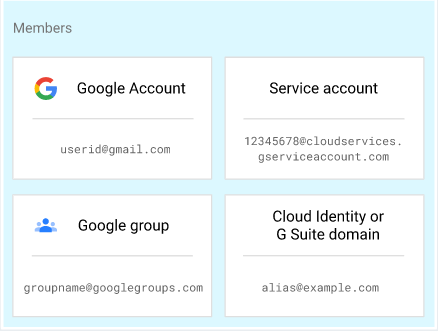
\includegraphics[width=\linewidth]{mem}
  \caption {Types of Members in GCP}
  \label{fig:mem}
\end{figure}



Member,role and policy are three main parts of the authorization process.
Instead of assigning permission directly to end user to access a resource, in Google Cloud, permissions are grouped into roles and roles are granted to authenticated members.  
A role is a collection of permissions determining what operations are allowed on a resource (Figure ~\ref{fig:role}). Granting a role to a member actually grants all the permissions of that the role. 
\begin{figure}[h]
  \centering
  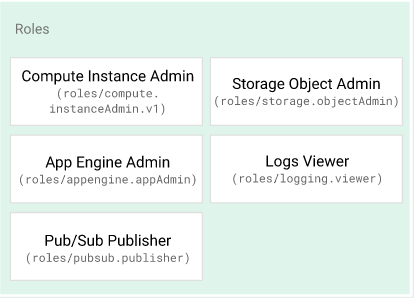
\includegraphics[width=\linewidth]{role}
  \caption {GCP Predefined Role}
  \label{fig:role}
\end{figure}
A policy binds who (member) has what access (role) for which resource \cite{Googlecloudiam}. Some examples of resources are organizations, folders, projects, Compute Engine instances, and Cloud Storage buckets. Multiple members can be bind to one role \cite{Googlecloudiam}. 
Primitive, predefined and custom roles are three types of roles supported in Google Cloud IAM \cite{googlecloudrole}. Primitive roles (renamed as Basic roles later) comprises Owner, Editor and Viewer roles, which exist prior to IAM in GCP. Predefined roles are finer-grained roles for a specific service . You can also limit privileges further by creating custom role and attach more specific permissions. This role based model of Google cloud IAM makes adopting the security Principle of Least Privilege straightforward.

For example, if a couple of users need to view all files and file content in a public bucket in the project. you can add every one to a Google group and grant the Storage Admin role (roles/storage.
admin) to the Google group. By looking through Table ~\ref{table:sto-role}, which displayed all predefined roles and their permissions associated with Cloud Storage, we notice that Storage Object Viewer would be sufficient to perform the same task. Therefore, binding Storage Object Viewer to the Google group would be a better option (Figure ~\ref{fig:sto-pre}). However, we know that the actual permissions needed are storage.objects.list (to list file) and storage.objects.get (to view file content). Following PoLP, we can create custom role and attach only those two permissions memtioned (Figure ~\ref{fig:sto-cus}).

Custom roles provide user-specified list of permissions across services. Unfortunately, not all permissions can be linked to Custom roles such as Datastore related permissions.


\begin{table}[t]
    \begin{center}
    \begin{tabular}{|p{4cm}|p{4cm}|}
    \hline
    Role & Permissions\\
    \hline
    \hline
    Storage Object Creator\par(roles/storage.objectCreator) &  resourcemanager.projects.get  \par resourcemanager.projects.list \par storage.objects.create \\ %% $\pm$ \\
    \hline
    Storage Object Viewer\par(roles/storage.objectViewer) & resourcemanager.projects.get\par resourcemanager.projects.list\par storage.objects.get\par storage.objects.list \\ %% $\pm$ \\
    \hline
    Storage Object Admin\par(roles/storage.objectAdmin) & resourcemanager.projects.get \par resourcemanager.projects.list\par storage.objects.*\\ %% $\pm$ \\
    \hline
    Storage HMAC Key Admin\par(roles/storage.hmacKeyAdmin) &storage.hmacKeys.*\\
    \hline
     Storage Admin\par(roles/storage.admin) &firebase.projects.get\par resourcemanager.projects.get\par resourcemanager.projects.list\par storage.buckets.*\par storage.objects.*\\
    \hline
    \end{tabular}
    \caption{IAM roles for Cloud Storage}
    \vspace{-0.20in}
    \label{table:sto-role}
    \end{center}
\end{table}


\begin{figure}[h]
  \centering
  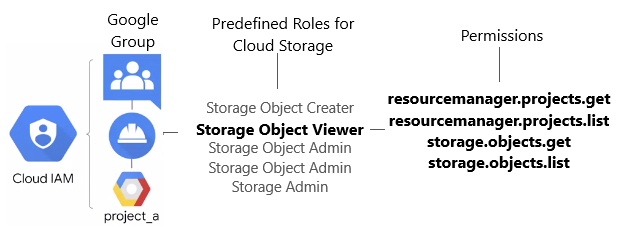
\includegraphics[width=\linewidth]{sto-pre}
  \caption {Policy - Predefined Role}
   \label{fig:sto-pre}
\end{figure}

\begin{figure}[h]
  \centering
  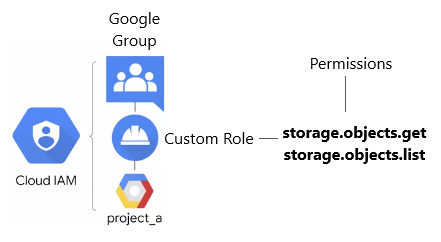
\includegraphics[width=\linewidth]{sto-cus}
  \caption {Policy - Custom Role}
   \label{fig:sto-cus}
\end{figure}




\section{Least Privilege CTF}

\subsection{Design Goal}
The purpose of Least Privilege CTF is to effectively teaching developers how to manage identity and access control and implement PoLP in Google Cloud project. Meanwhile, it should be able to run at minimum cost, deployed rapidly, extensible, friendly to beginners and delivered with instant feedback.

\begin{enumerate}
\item Minimum cost: Anyone can apply for 300 credits(dollars) for free with a Google account and credit card. If levels are deleted upon completion, monthly cost would be less than a dollar (Figure ~\ref{fig:cost}). 
\begin{figure}[h]
  \centering
  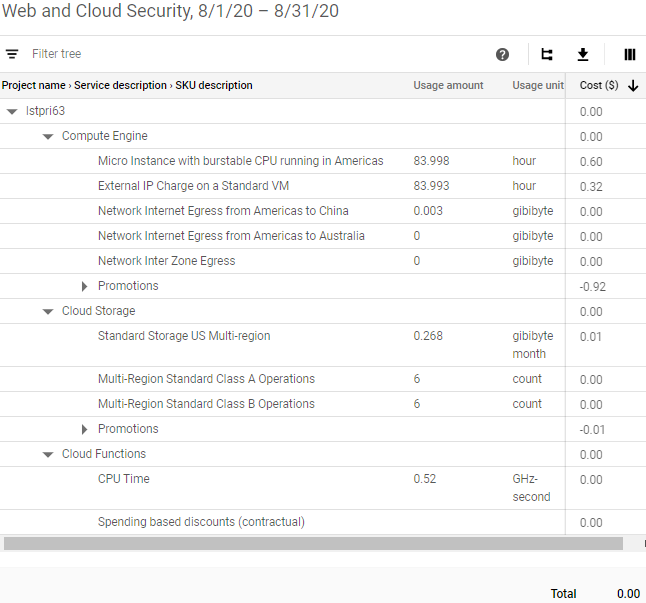
\includegraphics[width=\linewidth]{cost}
  \caption {Billing - Monthly Cost}
  \label{fig:cost}
\end{figure}
\item Fast Deployment: Google Cloud Deployment Manager deploys all required resources specified with a declarative format using yaml at one time in parallel. This feature enables initial 11 levels in 4.5 minutes.
\item Extensible: Easy to add new level with simple modification (Section 3.2.1).
\item Beginners friendly: Explicit and detailed instruction attached with each level that makes advance Google Cloud knowledge optional(Section 3.2.2).
\item Instant feedback: Results will be displayed immediately along with failing reason for each attempt (Section 3.2.2).

\end{enumerate}

\subsection{Implementation}

\subsubsection{Thunder CTF}
Least privilege CTF is developed from Thunder CTF, a scaffolded, scenario-based CTF that helps students learn about and practice cloud security skills on GCP. Each Thunder CTF level includes a yaml development configuration, a python deployment script and an HTML contents for hints \cite{Springer}. This specific structure reduces the process of creating or deprecating levels to simply updating existing templates. Least privilege CTF inherits modular structure from Thunder CTF, which allows levels to be added or removed easily with minimal code modification.

\subsubsection{UI and Cloud Functions}
Despite it takes a page \cite{lst-ctf} hosted under main Thunder CTF website for steps of environment set-up and initial deployment, Least Privilege CTF does not generate level hints with HTML contents or render scripts in a similar way as Thunder CTF does. Instead, level instructions and hints of Least Privilege CTF are established with Cloud Functions \cite{cloudfunc}, a pay-as-you-go service that automatically scales based on loads, meaning you are only billed for execution time. Cloud Functions demand no server management which speeds up the development as we do not have to deal with the operational infrastructure in Google Cloud. The integration of logging and debugging capabilities makes the coding experience intuitive. More importantly, Cloud Functions service has built in security at role per function based on PoLP. 

Least Privilge CTF selects HTTP functions \cite{httpfunc} that are invoked by standard HTTP requests and supports common methods like GET, PUT, POST, DELETE and OPTIONS to replace the hints system in Thunder CTF. A typical procedure in our design framework is that when a function is triggered by events, it waits for responses either returned from Cloud API or submitted in front-end using POST or GET method. The returned results are rendered into HTML through Jinja and reflect back to players. Thanks to the TLS certificates automatically provisioned in Cloud Functions service,  all HTTP functions can be invoked with a secure connection. 

In order to call a function and pass parameters, an URL known as HTTP-Triggered-Endpoint is obtained after each function deployment. Figure ~\ref{fig:endpoints} shows the function endpoints printed in Cloud Console shell when deployment manager completes the operation and creates initial levels.
Two python run time functions are written in each level, an access function (example Figure ~\ref{fig:access}) for listing step by step level instructions and resources, and a check function (example Figure ~\ref{fig:check}) for validating the correctness of the role attached to access function.Figure  ~\ref{fig:score} presents the Scoreboard Function that keeps track of the overall accomplishment.  
\begin{figure}[h]
  \centering
  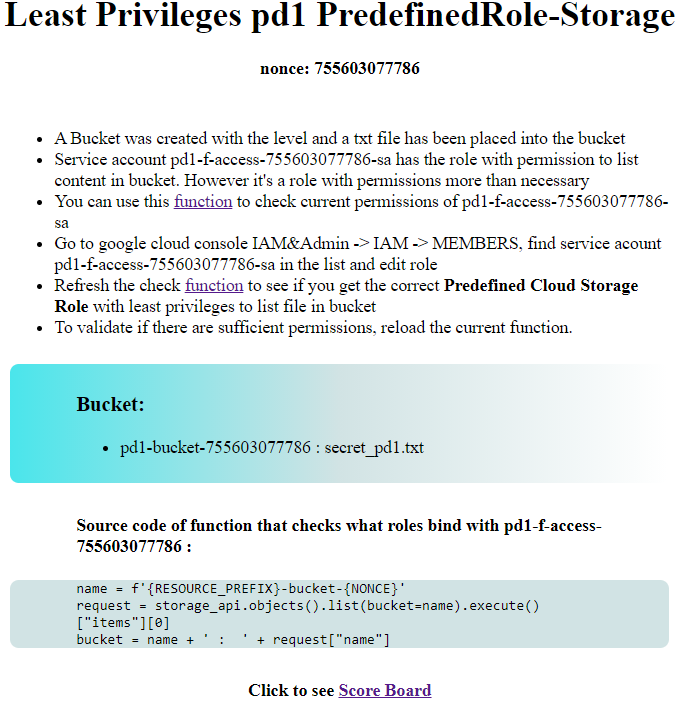
\includegraphics[width=0.5\textwidth]{access}
  \caption {Access Function}
  \label{fig:access}
\end{figure}
\begin{figure}[h]
  \centering
  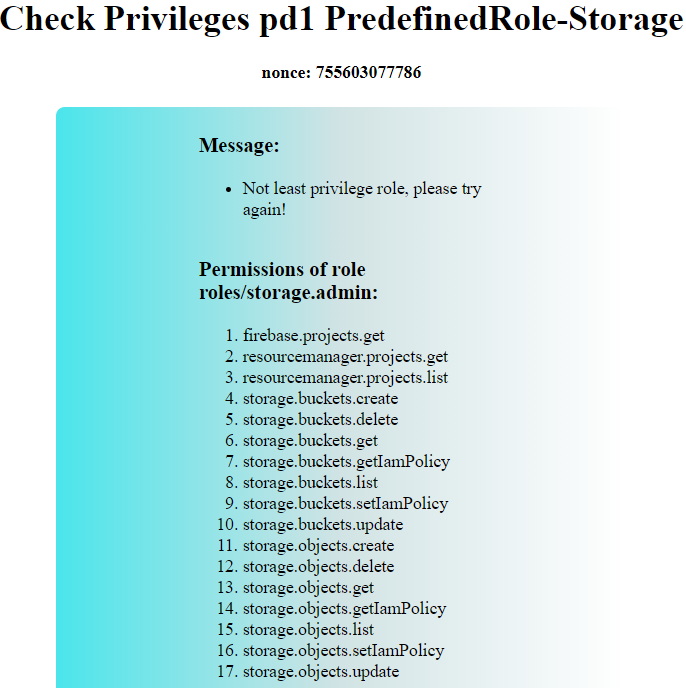
\includegraphics[width=0.5\textwidth]{check}
  \caption {Check Function}
  \label{fig:check}
\end{figure}

\begin{figure}[h]
  \centering
  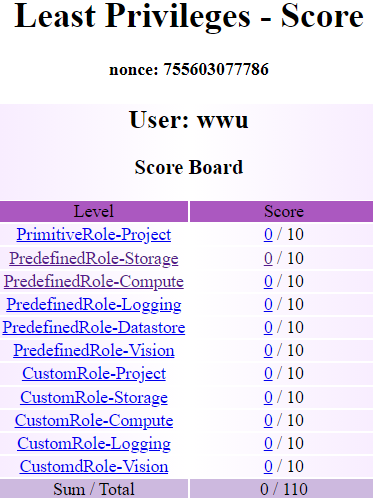
\includegraphics[width=0.4\textwidth]{score}
  \caption {Scoreboard Function}
  \label{fig:score}
\end{figure}

\begin{figure*}[h]
  \centering
  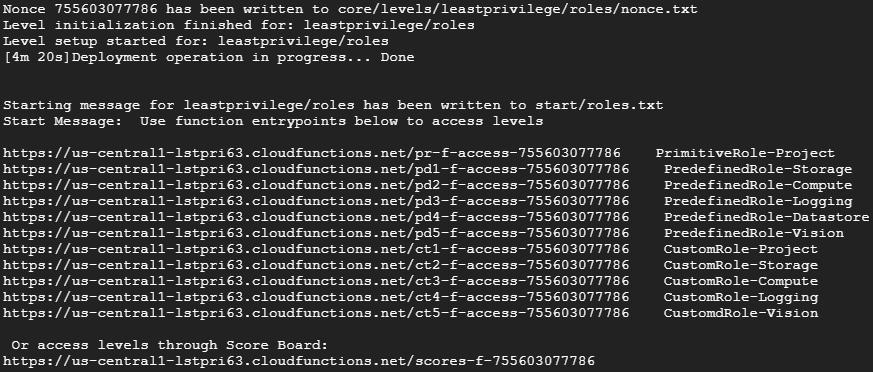
\includegraphics[width=0.7\textwidth]{endpoints}
  \caption {Endpoints}
   \label{fig:endpoints}
\end{figure*}
%%\begin{figure*}[t]
%%  \centering
 %% \begin{tabular}{c}
 %% 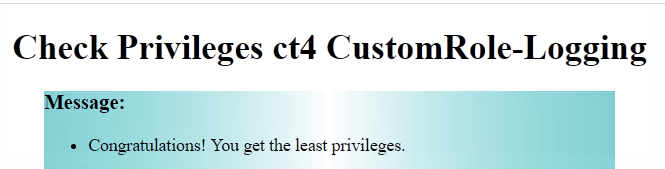
\includegraphics[width=0.60\textwidth]{success}
%%  \end{tabular}
%%\caption{Figure 1: function-validate answer and provide hints}
%%\label{fig:hints}
%%\end{figure*}
\subsubsection{Levels and examples}
Each Cloud function is expected to access level resources with its default service account. Service account of Check function only has privilege to list or get IAM permissions through API calls. All levels begin with a role attached to service account in Access Function,  containing excessive permissions,  to perform specific action. The winner condition is to modify the role with minimum permissions that performs the same action. 
Primitive roles, which include the Owner, Editor, and Viewer roles that existed prior to the introduction of IAM.
First level is designed for primitive role to list all resources in a project. Five levels are designed around predefined roles with different resources including cloud storage, vm instance, logging, datastore and cloud vision. Five levels are designed with custom role with corresponding resources, except that the datatore permissions are not supported in custom role.
\section{Evaluation}
 
The first use of Least Privilege CTF occurred in our Fall 2020 offering of Portland State University's CS 430/530 Internet, Web, and Cloud Systems course with 60 students.  The first half of the 10-week course covers key concepts in networking, operating systems, web development, and databases before transitioning to their use in cloud computing environments. At the beginning of the 6th week, a lecture on Google Cloud Identity and Access Management is given to students and the Least Privilege CTF levels were assigned. Students were given a due date for the exercises at the end of the 6th week, allowing them about a week to finish the levels.

To assess the effectiveness of the CTF, we surveyed students at the beginning of the 10th week. Below we list the questions that were asked in the survey in bullet points.  Our goal was to measure how well the CTF helped students learn about cloud security issues related to IAM and understand best practice.  

Questions included in the survey:
\begin{itemize}
\item Q1: Rate the CTF exercises for understanding security issues in the cloud.
\item Q2: Rate the CTF exercises for developing skills in navigating the cloud.
\item Q3: Rate the hint system as a mechanism for providing help as needed in solving CTF exercises.
\end{itemize}

Of the 60 students in the class, 36 responded to the survey.  Table~\ref{table:data} shows the results.  As the table shows, students felt that the lecture material and CTF exercises were both helpful for learning about security issues and for developing cloud skills, while students found the hint system very helpful as a learning aid, validating our design.


\begin{table}[t]
    \begin{center}
    \begin{tabular}{|l|l|l|l|l|l|l|}
    \hline
    Question & 1 & 2 & 3 & 4 & 5 &Mean rating\\
    \hline
    \hline
    Q1 & 1 & 3 & 3 & 19 & 10 & 3.94\\ %% $\pm$ \\
    \hline
    Q2 & 1 & 2 & 4 & 20 & 9 & 3.94\\ %% $\pm$ \\
    \hline
    Q3 & 1 & 0 & 1 & 10 & 24 & 4.56\\ %% $\pm$ \\
    \hline
    \end{tabular}
    \caption{Helpfulness ratings of Least Privilege CTF (1=Very Unhelpful, 2=Somewhat Unhelpful, 3=Neither Helpful nor Unhelpful, 4=Somewhat Helpful, 5=Very Helpful)}
    \vspace{-0.20in}
    \label{table:data}
    \end{center}
\end{table}

\section{Related Work}

Developers and researchers have actively worked on building cloud security CTF exercises or labs. Existing CTF platforms based on AWS including Flaws \cite{flaws}, Flaws2 \cite{flaws2}, CloudGoat \cite{cloudgoat}, OWASP ServerlessGoat \cite{serverlessgoat}. These platforms  demonstrate common security issues caused by various reasons throughout development, including authentication bypass and over-privileged access(misconfigured IAM). Most CTF exercises are offensive style, meaning the player will act as the attacker. It is the players’ mission to explore the environment, identify vulnerabilities, and exploit your way to the ‘secret’. Flaws2 contains both offensive and defensive style CTF exercises. Thunder CTF \cite{thunder-ctf} contains a extensive range of GCP (Google Cloud Platform) based labs, however best practice is not emphasized. QWIKLABS \cite{QWIKLABS} seems to be the only one who built security labs on both AWS and GCP environments. QWIKLABS designed courses and labs to help users gain cloud knowledge, practice building projects and get familiar with all the cloud services as quickly as possible. Although some QWIKLABS projects do require creating service account, attaching roles and granting permissions,  they issue temporary cloud credentials for players, so security is not one of their concern.

Existing services are available to help achieve least privilege with less effort through monitoring logs and configuration. For example, Google IAM Recommender \cite{GoogleLstRec} provides safe, in-context, and actionable changes to your IAM policies that move your project towards least privilege and don’t require lots of manual effort on your part. However, it will have to gather enough data to be able to make suggestions and establish best practice. This limitation makes Google IAM Recommender as well as a lot of other third party tools impractical for beginners to learn the concept of PoLP.
\section{Conclusion}

Identity and access management and following best practice are imperative in cloud security, however the concept of IAM and PoLP is difficult to understand. In this paper, we designed and implemented labs focused on enforcing the principle of least privilege in Google Cloud environment. The evaluation showed that results from an initial offering are promising and the design goals are achieved. 

\section{Acknowledgments}

This material is supported by the National Science Foundation under Grant No. 1821841. Any
opinions, findings, and conclusions or recommendations expressed in this material are those of the author and do not necessarily reflect the views of the National Science Foundation.



%%
%% The next two lines define the bibliography style to be used, and
%% the bibliography file.
\bibliographystyle{ACM-Reference-Format}
\bibliography{ref-base}

%%
%% If your work has an appendix, this is the place to put it.
\appendix


\end{document}
\endinput
%%
%% End of file `sample-lualatex.tex'.
